\textbf{ الاکلنگ بایاس و واریانس}

\begin{enumerate}[leftmargin=17pt]
\item 
تفاوت کاربرد داده‌های Validation و Test چیست؟
فقط به مهم‌ترین موضوع اشاره کنید.
\vspace{1cm}
\item 
فرض کنید قیمت یک رمزارز از تابع زیر تبعیت می‌کند:
$y=(1+sin(\frac{\pi x}{10}))+\epsilon$
که در آن 
$x$
شماره‌ی روز از ماه است. 
سه مدل زیر را در نظر بگیرید:
{\latin
\begin{itemize}
    \item $\hat{y_1}=\theta_1 x + \theta_0$
    \item $\hat{y_3}=\theta_3 x^3 + \theta_2 x^2 + \theta_1 x + \theta_0$
    \item $\hat{y_9}=\theta_9 x^9 + \cdots + \theta_2 x^2 + \theta_1 x + \theta_0$
\end{itemize}}
کم یا زیاد بودن مقدار 
Bias
و
Variance 
هریک از این سه مدل را در حالت‌های زیر با دلیل مشخص کنید. نیازی به محاسبات نیست.
\begin{itemize}
    \item
    وقتی ۱۰۰ داده از قیمت این رمزارز در طول یک ماه داریم.
    \vspace{2cm}
    \item
    وقتی ۵ داده از قیمت این رمزارز در طول یک ماه داریم.
    \vspace{2cm}
\end{itemize}

\item 
در شکل زیر محور 
$x$
تغییرات یک 
Hyperparameter
و محور 
$y$
مقدار تابع زیان Loss را نشان می‌دهد.
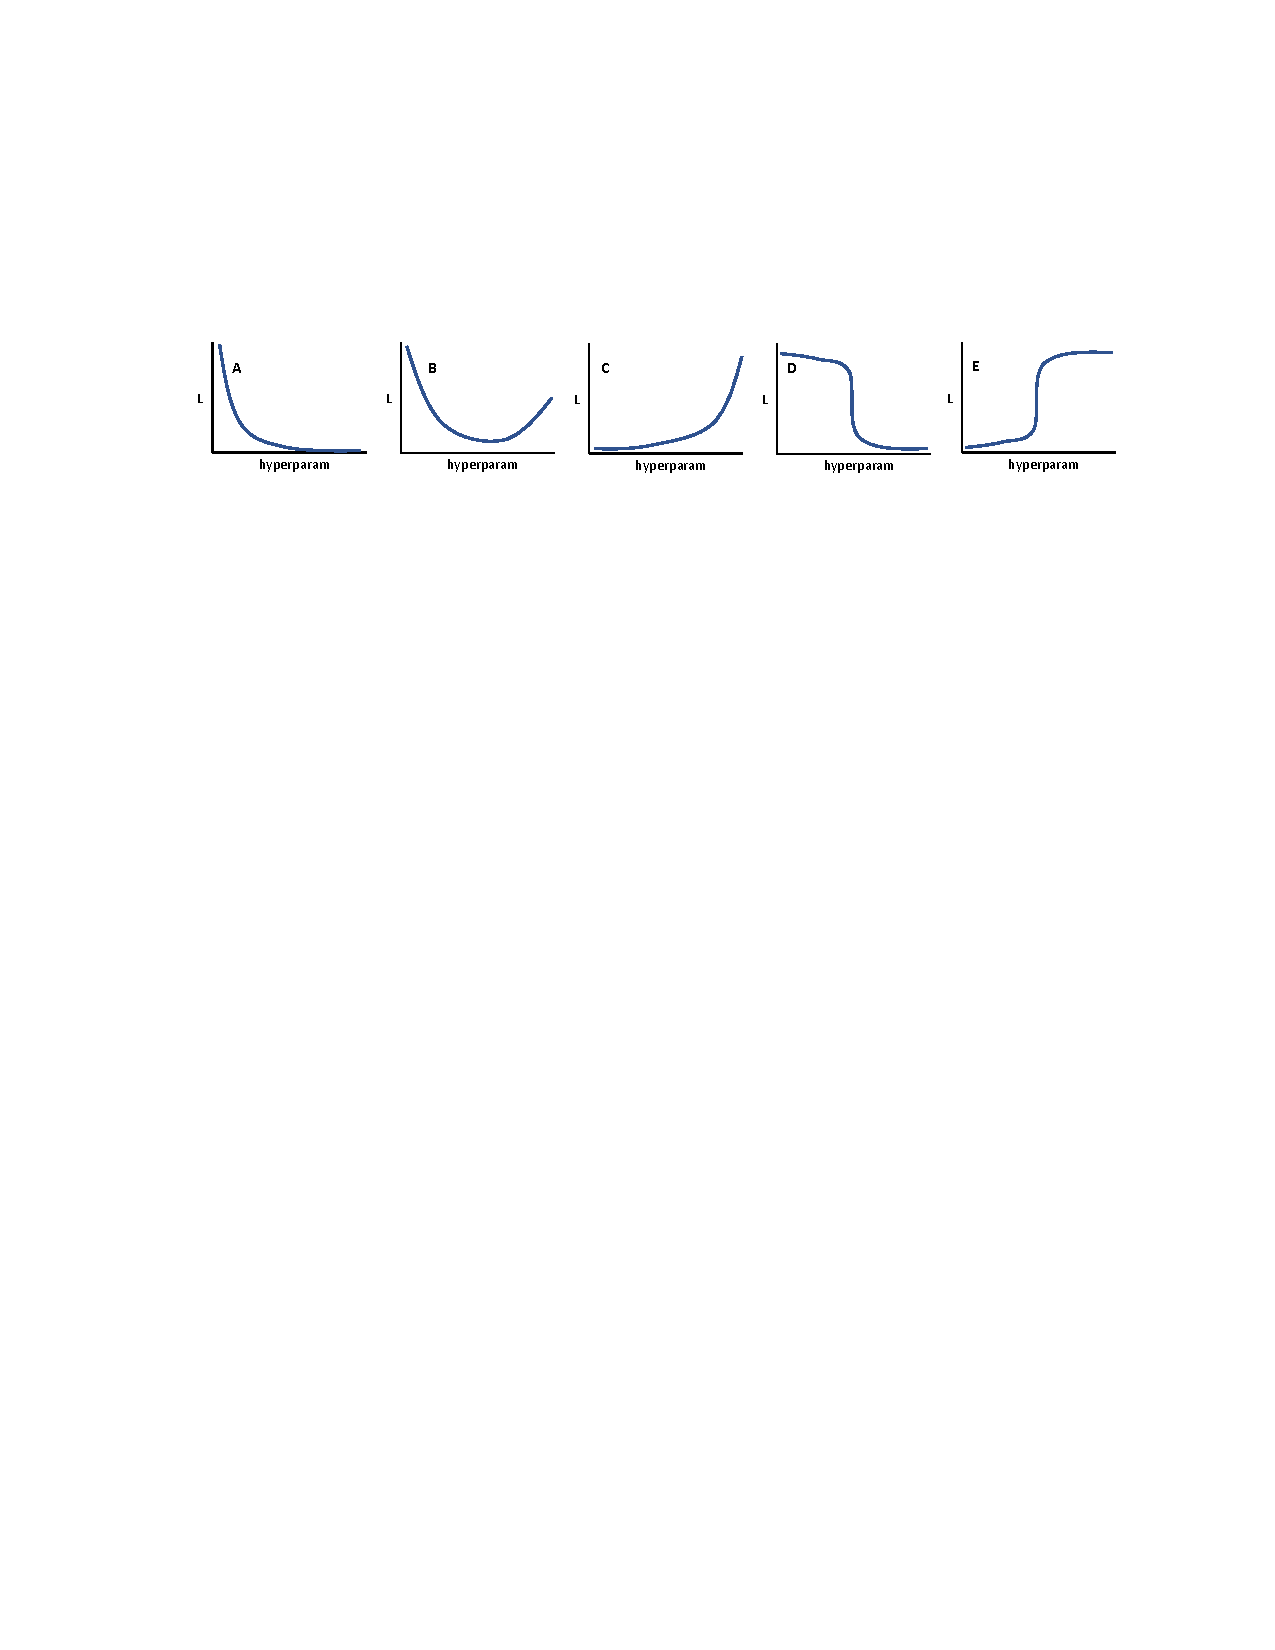
\includegraphics{images/1.pdf}
\vspace{1cm}

برای هریک از قسمت‌های زیر فقط یکی از شکل‌های A تا E را انتخاب کنید که محتمل‌ترین تغییر رفتار تابع زیان بر اساس تغییرات مقدار Hyperparameter
است. هم‌چنین، دلیل انتخاب خود را توضیح دهید.
\begin{enumerate}
    \item[(الف)] $k$: تعداد همسایگان در الگوریتم $k$ نزدیک‌ترین همسایه
    (kNN)
\begin{itemize}
        \item میزان خطا با تغییر $k$
{\latin      
\tikz\draw[thick](0,0)circle(0.15); A \quad
\tikz\draw[thick](0,0)circle(0.15); B \quad
\tikz\draw[thick](0,0)circle(0.15); C \quad
\tikz\draw[thick](0,0)circle(0.15); D \quad
\tikz\draw[thick](0,0)circle(0.15); E
}
\end{itemize}
\vspace{1.5cm}
\item[(ب)] $d$: عمق یک درخت تصمیم‌
\begin{itemize}
        \item زیان آموزش \lr{ Training Loss}
{\latin      
\tikz\draw[thick](0,0)circle(0.15); A \quad
\tikz\draw[thick](0,0)circle(0.15); B \quad
\tikz\draw[thick](0,0)circle(0.15); C \quad
\tikz\draw[thick](0,0)circle(0.15); D \quad
\tikz\draw[thick](0,0)circle(0.15); E
}
\vspace{1.5cm}
        \item زیان تست \lr{ Test Loss}
{\latin      
\tikz\draw[thick](0,0)circle(0.15); A \quad
\tikz\draw[thick](0,0)circle(0.15); B \quad
\tikz\draw[thick](0,0)circle(0.15); C \quad
\tikz\draw[thick](0,0)circle(0.15); D \quad
\tikz\draw[thick](0,0)circle(0.15); E
}
\vspace{1.5cm}
\end{itemize}
\item[(پ)] $\alpha$ نرخ یادگیری
\lr{Learning Rate}
در رگرسیون لاجستیک 
\lr{Logistic Regression}
\begin{itemize}
        \item زیان آموزش \lr{ Training Loss}
{\latin      
\tikz\draw[thick](0,0)circle(0.15); A \quad
\tikz\draw[thick](0,0)circle(0.15); B \quad
\tikz\draw[thick](0,0)circle(0.15); C \quad
\tikz\draw[thick](0,0)circle(0.15); D \quad
\tikz\draw[thick](0,0)circle(0.15); E
}
\vspace{1.5cm}
        \item زیان تست \lr{ Test Loss}
{\latin      
\tikz\draw[thick](0,0)circle(0.15); A \quad
\tikz\draw[thick](0,0)circle(0.15); B \quad
\tikz\draw[thick](0,0)circle(0.15); C \quad
\tikz\draw[thick](0,0)circle(0.15); D \quad
\tikz\draw[thick](0,0)circle(0.15); E
}
\vspace{1.5cm}
\end{itemize}

\item[(ت)] تعداد درختان در جنگل تصادفی \lr{Random Forest}
\begin{itemize}
        \item زیان آموزش \lr{ Training Loss}
{\latin      
\tikz\draw[thick](0,0)circle(0.15); A \quad
\tikz\draw[thick](0,0)circle(0.15); B \quad
\tikz\draw[thick](0,0)circle(0.15); C \quad
\tikz\draw[thick](0,0)circle(0.15); D \quad
\tikz\draw[thick](0,0)circle(0.15); E
}
\vspace{1.5cm}
        \item زیان تست \lr{ Test Loss}
{\latin      
\tikz\draw[thick](0,0)circle(0.15); A \quad
\tikz\draw[thick](0,0)circle(0.15); B \quad
\tikz\draw[thick](0,0)circle(0.15); C \quad
\tikz\draw[thick](0,0)circle(0.15); D \quad
\tikz\draw[thick](0,0)circle(0.15); E
}
\vspace{1.5cm}
\end{itemize}

\end{enumerate}
\end{enumerate}
